% Talk about software engineering practices for scientific workflows
% Ariel Rokem
% License: CC(http://creativecommons.org/licenses/by-nc-sa/3.0/)

\documentclass{beamer}

\usepackage{ulem}
\usepackage{listings,bera}
\usepackage{graphics}
\usepackage{media9}

\setbeamercovered{transparent}
\usetheme{CambridgeUS}
\usecolortheme{beaver}
\useinnertheme{rectangles}

\definecolor{fore}{RGB}{0,20,30}
\definecolor{back}{RGB}{255,255,255}
\definecolor{title}{RGB}{140,21,21}

\setbeamercolor{titlelike}{fg=title}
\setbeamercolor{normal text}{fg=fore,bg=back}
\definecolor{keywords}{RGB}{255,0,90}
\definecolor{comments}{RGB}{60,179,113}
\definecolor{strings}{RGB}{120,120,0}

\lstset{language=Python,
keywordstyle=\color{keywords},
commentstyle=\color{comments}\emph,
stringstyle=\color{strings}}

\title[Practical software engineering]{Practical software engineering }
\subtitle{for psychologists}

\author[Ariel Rokem]
{Ariel Rokem}
\date{October 17, 2014}
\institute[Stanford University]
{Stanford University}

% Put in stanford and vista logos:
\pgfdeclareimage[height=1.5cm]{stanford-logo}{figures/stanford_logo}
\setbeamertemplate{itemize}
  
\begin{document}

%Title page:
\begin{frame}
  \titlepage
  \pgfuseimage{stanford-logo}

\end{frame}

\begin{frame}
\frametitle{"Dammit Jim, I'm a psychologist, not a programmer!''}
\begin{itemize}
\pause
\item
Humans are good at many things
\pause
\item 
Computers are good at other things
\pause
\item
Automate everything you can
\pause
\item
Now, we've settled that, how can we make sure we do it well? 
\end{itemize}
\end{frame}

\begin{frame}
\frametitle{Make your life easier}
\pause
And your results easier to reproduce
\end{frame}

\begin{frame}
\pause
Reproducibility is collaborating with someone you don't yet know
\pause 
... Yourself in a couple of months, for example
\end{frame}

\begin{frame}
\frametitle{3 practices you can adopt}
\begin{itemize}
\pause
\item
Version control
\pause
\item
Testing
\pause
\item
Code review 
\end{itemize}
\end{frame}

\begin{frame}
\frametitle{3 practices you can adopt}
\begin{itemize}
\item
\emph{Version control}
\item
Testing
\item
Code review 
\end{itemize}
\end{frame}

\begin{frame}
\frametitle{Version control}
Who uses version control?
\end{frame}

\begin{frame}
\frametitle{We all do}
 
\includegraphics[height=5.7cm]{figures/vcs_for_science.png}
\end{frame}


\begin{frame}
\frametitle{Wouldn't you rather be more systematic?}
There are many Version Control Systems
\begin{itemize}
\pause
\item
SVN
\pause
\item
CVS 
\pause
\item
GIT
\end{itemize}
\end{frame}


\begin{frame}
\frametitle{Git}
Created by Linus Torvalds
\begin{itemize}
\pause
\item
Distributed
\pause
\item
Fast 
\pause
\item
In very common use
\end{itemize}
\end{frame}

\begin{frame}
\frametitle{What it does}
Git keeps snapshots of your file system
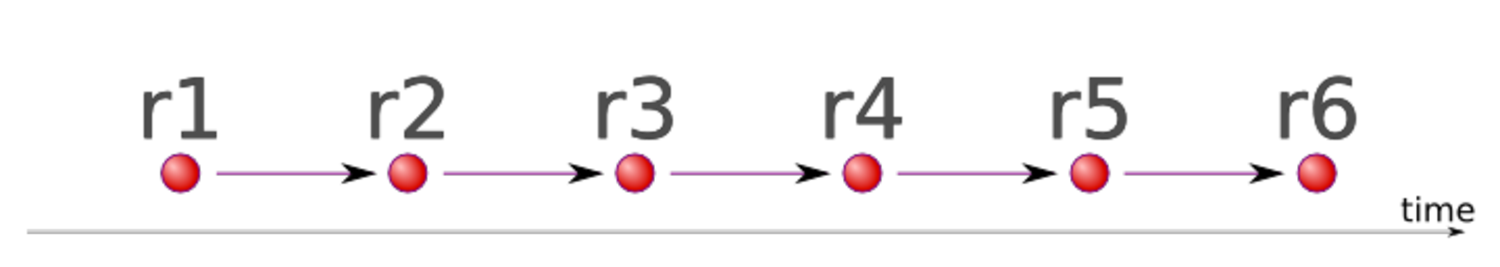
\includegraphics[height=2cm]{figures/git1.pdf}
\end{frame}

\begin{frame}
\frametitle{What it does}
You can revert back to a previous version
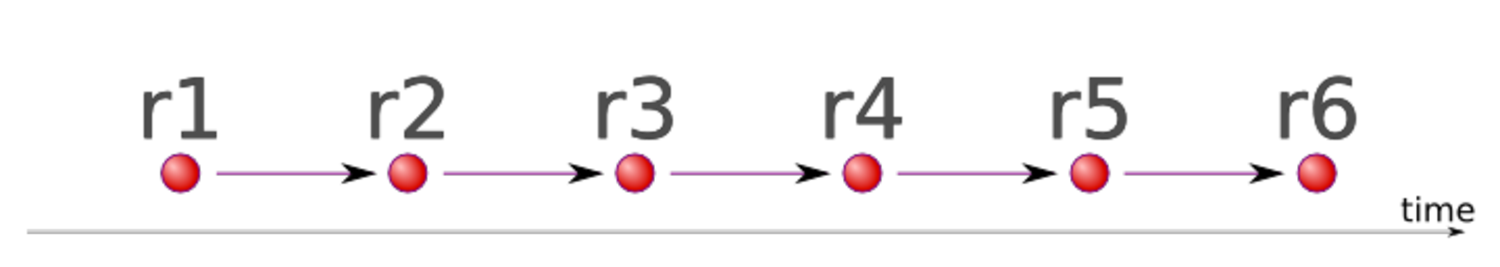
\includegraphics[height=2cm]{figures/git1.pdf}
\end{frame}

\begin{frame}
\frametitle{Easy to branch}
This is a way to try out new ideas
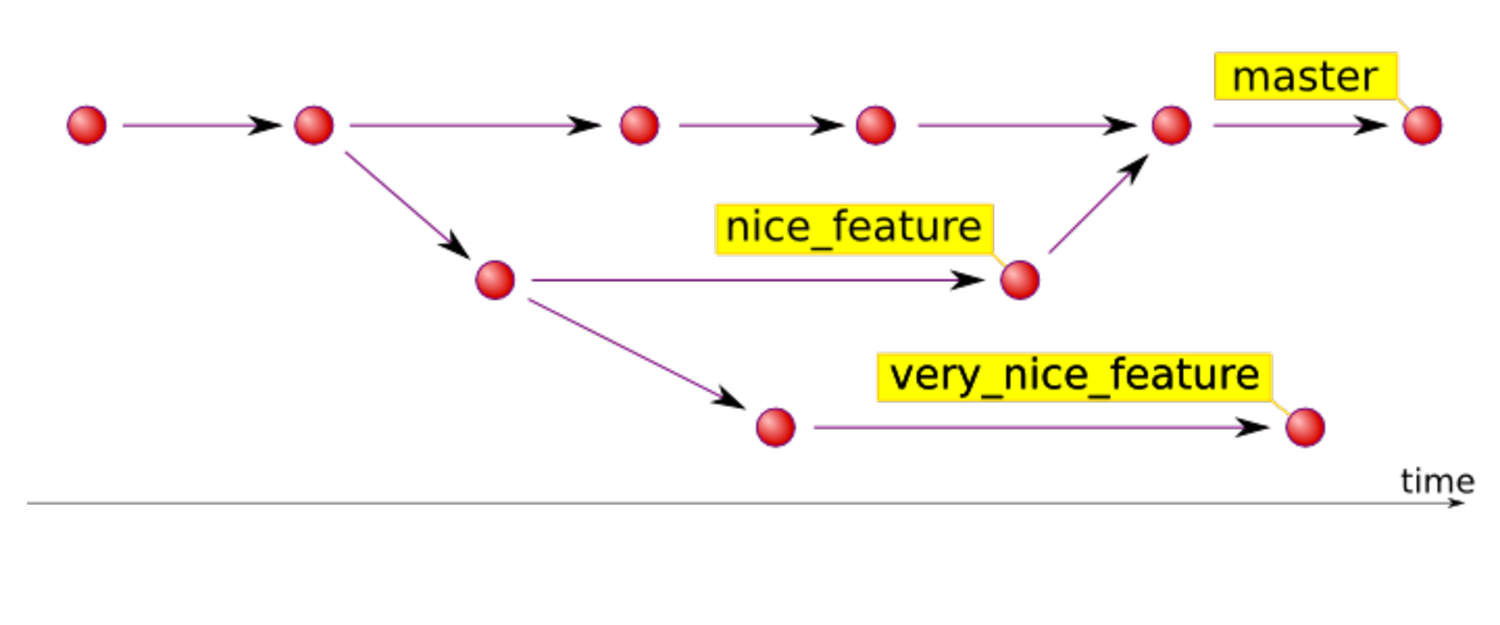
\includegraphics[height=4cm]{figures/git2.pdf}
\pause
\\
Without worrying you might break something
\end{frame}

\begin{frame}
\frametitle{An easy backup system}

With annotation built in

\end{frame}

\begin{frame}

The modern lab notebook?

\end{frame}


\begin{frame}
\frametitle{Collaboration is easy}
\begin{itemize}
\pause
\item
Github 
\pause
\item
\href{https://education.github.com/}{Github for students}
\end{itemize}
\end{frame}


\begin{frame}
\frametitle{Version everything!}
\begin{itemize}
\pause
\item
Code
\pause
\item
Papers
\pause
\item
Data (of reasonable size)
\pause 
\item
Even presentations
\pause
\item
\href{https://github.com/arokem/frisem-20141016}{This talk}
\end{itemize}
\end{frame}


\begin{frame}
\frametitle{3 practices you can adopt}
\begin{itemize}
\item
Version control
\item
\emph{Testing}
\item
Code review 
\end{itemize}
\end{frame}


\begin{frame}
\frametitle{Automated testing}
How do you know your code does what it's supposed to do?
\pause
How do you prevent bugs from recurring?
\pause 
How do you avoid breaking old functions, when building new ones?
\end{frame}

\begin{frame}[fragile]
\frametitle{Assert simple test cases}
\begin{lstlisting}
def circle_diameter(radius):
  return(2 * pi * radius)
\end{lstlisting}
\end{frame}

\begin{frame}[fragile]
\frametitle{Assert simple test cases}
\begin{lstlisting}

def test_circle_diameter(radius):
    assert circle_diameter(2) == 2 * pi

\end{lstlisting}
\end{frame}

\begin{frame}[fragile]
\frametitle{Assert simple test cases}
If it gets those wrong -- 
\\ 
it certainly will not do well with more complicated things!
\end{frame}


\begin{frame}[fragile]
\frametitle{Assert your old results}

Regression testing

\end{frame}


\begin{frame}[fragile]
\frametitle{Assert fixes to bugs}

Those tend to creep back in somehow 

\end{frame}



\begin{frame}
\frametitle{The benefits of tests}
\begin{itemize}
\pause
\item
Validation
\pause
\item
Avoid regressions
\pause
\item
Documentation
\end{itemize}
\end{frame}

\begin{frame}
\frametitle{The benefits of tests}
Don't let this happen to you
\\

\includegraphics[height=6cm]{figures/lack_of_tests.jpg}
\end{frame}

\begin{frame}
\frametitle{Continuous integration}
Have your version control system run your tests for you

\href{https://travis-ci.org}{Travis}

\end{frame}

\begin{frame}
\frametitle{3 practices you can adopt}
\begin{itemize}
\item
Version control
\item
Testing
\item
\emph{Code review}
\end{itemize}
\end{frame}


\begin{frame}
\frametitle{Code review}
\begin{itemize}
\pause
\item
Rigor
\pause
\item
Reusability
\pause
\item
Knowledge transfer
\end{itemize}
\end{frame}


\begin{frame}
\frametitle{How to make review work (author)}
\begin{itemize}
\pause
\item
 Less than 200 loc
\pause
\item 
 Digestible, coherent piece of code
\pause
\item
 Explain in advance what you are trying to achieve
\pause
\item 
 Write tests
\pause
\item
 Readability counts!\footnotemark[1]
\end{itemize}
\footnotetext[1]{\href{http://legacy.python.org/dev/peps/pep-0020/}{The zen of python}}
\end{frame}

\begin{frame}
\frametitle{How to make review work (reviewer)}
\begin{itemize}
\pause
\item 
Have clear standards
\pause 
\item 
Don't accept broken windows and technical debt
\pause
\item 
Don't forget to be positive
\pause
\item 
Readability counts! 
\end{itemize}
\end{frame}

\begin{frame}
\frametitle{Take breaks}
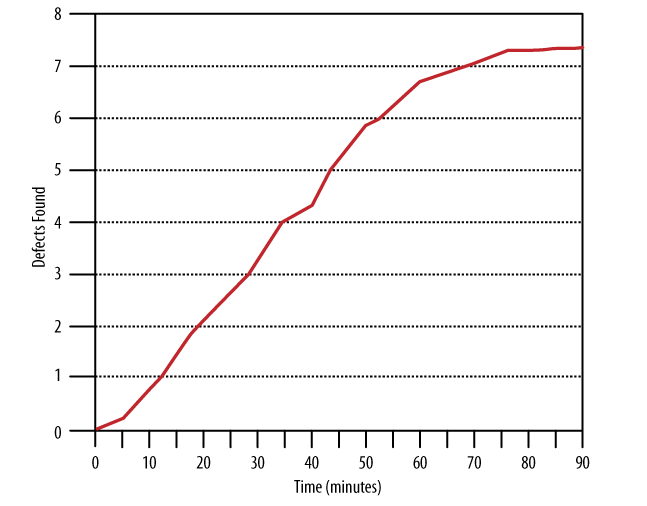
\includegraphics[height=6cm]{figures/review_errors}
\end{frame}


\begin{frame}
\frametitle{Modes of code review}
\begin{itemize}
\pause
\item
Asynchronous 
\pause
\item
Synchronous 
\end{itemize}
\end{frame}

\begin{frame}
\frametitle{Asynchronous: github pull requests}
\begin{itemize}
\pause
\item
Author creates a branch with proposed changes 
\pauses
\item
Author submits Pull Request through the web interface
\pause
\item
Reviewer reads and comments
\pause
\item
Author revises code
\pause
\item
Et cetera
\end{itemize}
\end{frame}

\begin{frame}
\frametitle{Synchronous: journal club/lab meeting for code}
\begin{itemize}
\pause
\item
Rob Knight, CU Boulder \footnotemark[1]
\pause
\item
Code is sent in advance (through github?)
\pause
\item 
Project on a screen and fire away!
\end{itemize}
\footnotetext[1]{\href{http://fperez.org/py4science/code_reviews.html}{h/t Fernando
  Perez}}
\end{frame}

\begin{frame}
\frametitle{When in doubt}
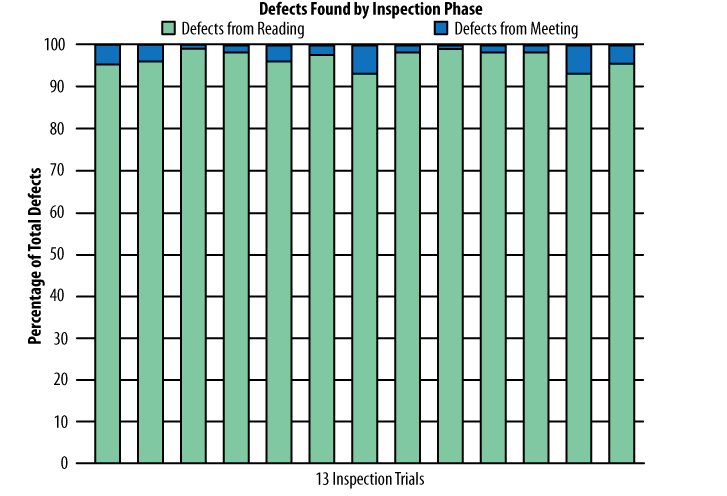
\includegraphics[height=5.7cm]{figures/review_meetings.png}
\end{frame}

\begin{frame}
\frametitle{Final thoughts}
\begin{itemize}
\pause
\item
Don't let the perfect be the enemy of the good

\pause
\item
Don't let the perfect be the enemy of the good

\end{itemize}
\end{frame}


\end{document}
